\section{Background}
\label{sec:background}

\subsection{Existing IoT Ecosystems}
\label{sec:iot-ecosystems}

Many current IoT architectures and frameworks, such as Bluetooth~\cite{bluetooth}, ZigBee~\cite{zigbee}, and Google Thread~\cite{thread}, have primarily focused on achieving device-to-device connectivity and interoperability.
For example, Bluetooth defines a seven-layer protocol stack and how two devices can connect to each other over either point-to-point or mesh networks, discover the other's capabilities through application layer profiles, and exchange application data called attributes.
Designed as silos, these architectures cannot interoperate with each other without special gateway or translator deployed in between, limiting development and innovation of IoT technologies.

% JB: How does preceding sentence and this paragraph relate to overall thesis of paper? 
As the IoT systems become more powerful and more complex, there is a growing demand for more comprehensive application-layer frameworks that can integrate and manage different types of devices across different communication technologies, enable more intelligent application logic involving a large number of devices, and provide simplified user experience in operating such systems.
In this subsection, we briefly review a few popular IoT application frameworks that appeared in the last three years.

\emph{AllJoyn}~(2013\footnote{The number in parentheses indicates the year of initial public announcement.})~\cite{alljoyn} and \emph{IoTivity}~(2015)~\cite{iotivity} are generic IoT application frameworks that aim at bridging various IoT transport technologies and providing a common language for the applications and services.
They both provide standardized interfaces for common IoT services such as device management, resource discovery, application-layer messaging, access control, etc.
While they started with an emphasis on proximal (i.e., local-area) communications, they also define gateway interfaces for connecting to external services both locally and in the cloud.
% These two frameworks are \emph{cloud-neutral} in the sense that they support but do not mandate the cloud as part of the IoT system.
As lower-level frameworks, they do not mandate specific solutions for trust management and rendezvous, but provide common protocol interfaces for developers to design and implement applications and services that run either locally or remotely in the cloud.
%\hl{For the purposes of this paper, it is important to note that they must handle the mapping of named entities to host-based addressing.}

\emph{AWS IoT}~(2015)~\cite{aws-iot}, \emph{Google Weave}~(2015)~\cite{weave}, \emph{Azure IoT Suite}~(2015)~\cite{azure-iot}, and \emph{Samsung SmartThings}~(2014)~\cite{smartthings} are examples of \emph{cloud-centric} IoT ecosystems that are bound to specific cloud service providers and their implementations of all common IoT services, from authentication and device management to data processing and application hosting.
Through tight integration with the cloud, those ecosystems provide simple and centralized solutions for trust management and rendezvous.
The user typically registers all local IoT devices and applications with the remote cloud service.
The cloud then handles the complex tasks of authentication and maintaining a complete catalog of available functionality in the local environment, so that devices and applications can securely discover and communicate with each other.
Another benefit of such cloud-centric architectures is easy integration with higher-level services such as search, voice recognition, and  data analytics, which are beneficial to large-scale IoT systems including precision agriculture and industrial control.

A notable recent trend among such cloud-centric architectures has been to move certain IoT applications and services into the local network and execute them on a local \emph{hub} in order to tolerate intermittent cloud connectivity.
For example, Amazon, Google, and Samsung all created their own home hub devices to connect local IoT devices and perform simple home automation tasks.
The recently announced \emph{AWS Greengrass}~(2016)~\cite{aws-greengrass} even allows part of the AWS IoT control plane to be hosted on a local server, essentially creating a private cloud service close to the IoT deployment.
However, local data (e.g., device state, system config, etc.) still need to be synchronized to the remote cloud to be consumed by cloud-hosted services.

\emph{Apple HomeKit}~(2014)~\cite{homekit} is an IoT framework designed specifically for home automation applications running on Apple devices.
Different from the cloud-centric ecosystems mentioned above, the HomeKit design enables and encourages local communication.
The framework stores the home configuration in a local database which is synchronized across all the devices that belong to or are authorized by the same user.
After obtaining permissions from the user, HomeKit applications on any of those devices can access the database to discover and control the home devices directly over the local network.
Hence, the rendezvous service is provided locally through database synchronization so that each device has complete knowledge of the home network.
However, HomeKit still relies on Apple's iCloud service for trust management: all new users and devices must be authenticated with Apple and obtain iCloud IDs.
While the replication of the home database allows rendezvous to be performed locally, the synchronization of the database across devices is done indirectly via iCloud.
Moreover, remote control requires tunneling the control messages through iCloud to a local hub (e.g., an Apple TV)
 inside the home network.

Table~\ref{tab:existing-ecosystems} summarizes approaches that different IoT architectures and ecosystems take in providing the trust management and rendezvous services.
Note that all of them are built on top of TCP/IP architecture and therefore have to provide the mapping services that resolve named entities to host-based addresses, either remotely in the cloud DNS service or locally via some zero-conf protocol such as mDNS.

\begin{table}[!t]
\renewcommand{\arraystretch}{1.3}
\caption{Comparison of existing IoT architectures and ecosystems.}
\label{tab:existing-ecosystems}
\centering
\begin{tabular}{|c|c|c|}
\hline
 & Trust management & Rendezvous\\
\hline
Bluetooth & P2P peering & None (P2P)\\
\hline
ZigBee & Pre-shared master key & Broadcast\\
\hline
Google Thread & L2 network-wide key & None\\
\hline
AllJoyn / IoTivity & Interface only & Interface only\\
\hline
AWS IoT & Cloud service & Cloud service\\
\hline
Google Weave & Cloud service & Cloud service\\
\hline
Azure IoT Suite & Cloud service & Cloud service\\
\hline
Samsung SmartThings & Cloud service & Cloud service\\
\hline
Apple HomeKit & Cloud service & Local database sync\\
\hline
\end{tabular}
\end{table}


\subsection{Named Data Networking of Things}

\emph{Named Data Networking (NDN)} is a proposed future Internet architecture.
%Compared to the existing TCP/IP architecture, 
NDN replaces host-addressed IP packets with named data as the new narrow waist of the hourglass protocol stack.
Each data object has a hierarchical name that serves as the unique identifier within the context of application where the data is published and consumed.
To request a data object, the consumer sends an \emph{Interest} packet carrying a prefix of the data name.
 NDN forwarders forward the Interest packet towards the locations where the data may be found.
Each forwarder along the path records the Interest and its incoming interface in the local \emph{Pending Interest Table (PIT)}.
When a matching \emph{Data} packet is encountered, either in the forwarder cache or the original producer, the Data packet is returned to the consumer by following the reverse path of the Interest recorded in PIT.
The nodes that have forwarded the Data packet store the data in their local caches, which can be used to satisfy future requests.
The Data packet carries a cryptographic signature generated by its producer, and information about how to retrieve the signing key (or key certificate).
This allows the consumer to verify the provenance of the data regardless of its source.

%JB: The paper below should be cited earlier. 
In our previous paper~\cite{ndn-iot} we described how NDN provides a more secure and straightforward solution for IoT networking (compared to TCP/IP) by naming and securing the \emph{things} and their data directly at the network layer:
\begin{itemize}
\item The Interest-Data exchange model in NDN closely resembles the RESTful protocols such as HTTP and CoAP that are widely adopted in the IoT applications.
\item Name-based forwarding simplifies the network stack by removing the extra step of resolving application names to network identifiers (e.g., IP and MAC addresses).
\item Data-centric security is more efficient and IoT-friendly than the channel- or isolation-based alternatives.
\item The ubiquitous data caching in the network also improves the efficiency of information dissemination especially for constrained IoT environments.
\end{itemize}
We also described various higher-level protocols built on top of NDN to achieve framework functionalities such as bootstrapping and discovery, trust management, access control, multi-party communication, and global integration.
We refer readers to~\cite{ndn-iot} for complete discussion.
The major differences between NDN- and IP-based IoT architectures are illustrated in Fig.~\ref{fig:ndnot-vs-iot}.

\begin{figure}[!t]
\centering
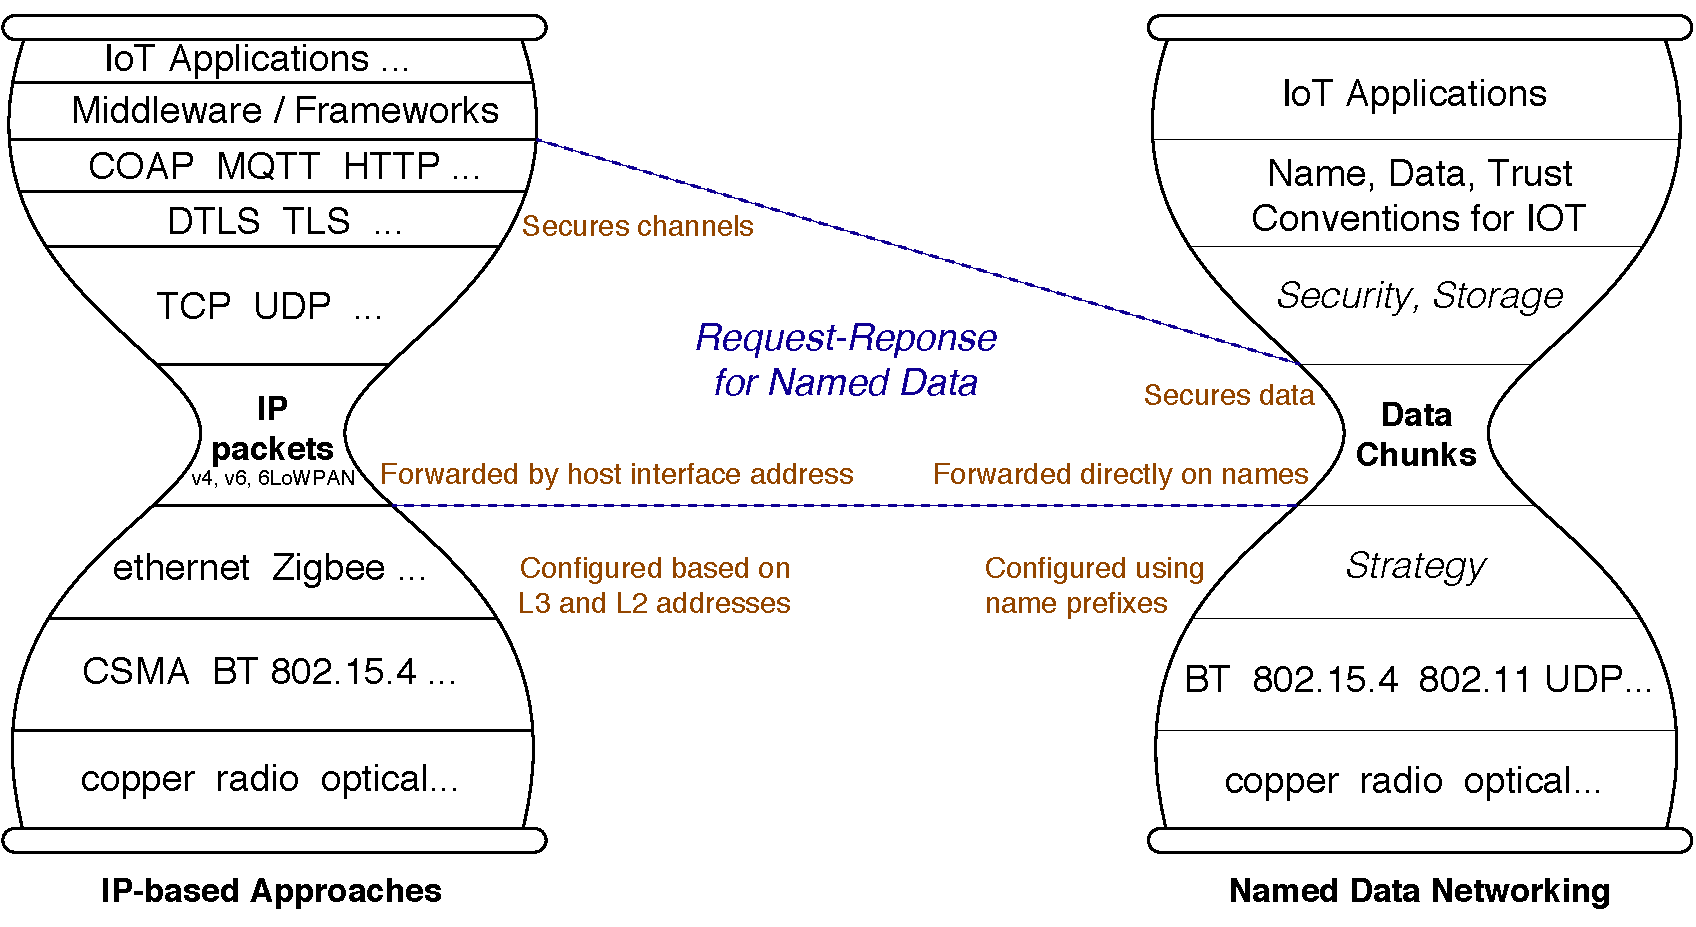
\includegraphics[width=0.9\columnwidth]{ndn-iot-hourglass.pdf}
\caption{Protocol stack comparison of NDN and TCP/IP.}
\label{fig:ndnot-vs-iot}
\end{figure}

The goal of this paper is to demonstrate the design and implementation of a complete IoT system based on NDN, expanding on our previous work.
In particular, we will illustrate how to leverage naming in NDN to achieve trust management and rendezvous in an IoT network, which further enables a variety of IoT applications and services.
